\documentclass[12pt,letterpaper]{article}
\usepackage{fullpage}
\usepackage[top=2cm, bottom=4cm, left=2cm, right=2cm]{geometry}
\usepackage{amsmath,amsthm,amsfonts,amssymb,amscd}
\usepackage{lastpage}
\usepackage{enumerate}
\usepackage{fancyhdr}
\usepackage{mathrsfs}
\usepackage{xcolor}
\usepackage{graphicx}
\usepackage{listings}
\usepackage{hyperref}
\usepackage{siunitx} % Formats the units and values
\usepackage{appendix}
\usepackage{caption}
\usepackage{subcaption}
\usepackage{multicol}
\usepackage{wrapfig}
\usepackage{esint}
\usepackage[utf8]{inputenc}
\usepackage[T1]{fontenc}
\usepackage[inline]{enumitem} %allows inline itemize or enumerate
\usepackage{pdfpages}
\usepackage{booktabs} % For \toprule, \midrule and \bottomrule
\usepackage{pgfplotstable} % Generates table from .csv
\pgfplotsset{compat=1.16}
% Setup siunitx:
 \sisetup{
   round-mode          = places, % Rounds numbers
   round-precision     = 2, % to 2 places
 }


\hypersetup{%
  colorlinks=true,
  linkcolor=blue,
  linkbordercolor={0 0 1}
}
 
\renewcommand\lstlistingname{Algorithm}
\renewcommand\lstlistlistingname{Algorithms}
\def\lstlistingautorefname{Alg.}

\lstdefinestyle{Python}{
    language        = Python,
    frame           = lines, 
    basicstyle      = \tiny,
    keywordstyle    = \color{blue},
    stringstyle     = \color{green},
    commentstyle    = \color{orange}\ttfamily
}

\setlength{\parindent}{0.0in}
\setlength{\parskip}{0.1in}
\setlength{\tabcolsep}{6pt}

%Astronomical units
\DeclareSIUnit \parsec  {pc}
\DeclareSIUnit \year    {yr}

% Edit these as appropriate
\newcommand\course{ASTRO 732}
\newcommand\coursename{Computational Methods for Astrophysics}
% \newcommand\course{ASTRO 645}
% \newcommand\coursename{Astrophysical Dynamics}
\newcommand\hwnumber{5}
\newcommand\myname{Sandra Bustamante}  
%allows to number the last equation of align.
\newcommand\numberthis{\addtocounter{equation}{1}\tag{\theequation}}

\pagestyle{fancyplain}
\headheight 35pt
\lhead{\course \\ Homework \hwnumber}
\chead{\textbf{\Large Liouville and Boltzmann}}
%\rhead{\myname \\ Due October 29, 2019}
\rhead{\myname}
\lfoot{}
\cfoot{\coursename}
\rfoot{\small\thepage}
\headsep 1.5em

%redefines subsections to be letters instead of numbers so 1.a normal way is 1.1
% \arabic (1, 2, 3, ...)
% \alph (a, b, c, ...)
% \Alph (A, B, C, ...)
% \roman (i, ii, iii, ...)
% \Roman (I, II, III, ...)
\renewcommand\thesubsection{\thesection.\alph{subsection}}

%%%%%%%%%%%%%%%%%%%%%%%%%%%%%%%%%%%%%%%%%%%%%%%%%%%%%%%%%%%%%%%
%=====================BEGIN DOCUMENT===========================
%%%%%%%%%%%%%%%%%%%%%%%%%%%%%%%%%%%%%%%%%%%%%%%%%%%%%%%%%%%%%%%

\begin{document}
\twocolumn
\lstset{style=Python}

% textwidth is \the\textwidth \\
% column width is \the\columnwidth \\
% textheight is \the\textheight

\section{Gauss-Laguerre Integration}

The convolution of an exponential decay and a Gaussian resolution function is given by
\begin{equation}
    f(t)=\int^\infty_0 \frac{e^{\frac{-(t-t')^2}{2\sigma^2_t}}}{\sqrt{2\pi\sigma^2_t}}\frac{e^{\frac{-t'}{\tau}}}{\tau}dt'.
    \label{eq:convolution}
\end{equation}

This can be integrated using Gauss-Laguerre Integration. It consists of making the integral into the form:
\begin{equation}
    f(t)=\int^\infty_0 dx w(x) f(x)
\end{equation}
where $w(x)$ is of the form $e^{-x}$. To achieve this form we have to make the following substitution $x=t'/\tau$ and $dx=dt'/\tau$. Then we have the following
\begin{align*}
    f(x)&=\frac{1}{\sqrt{2\pi\sigma_t^2}}\int^\infty_0 e^{-\frac{(t-x\tau)**2}{2\sigma_t^2}}e^{-x} dx\\
    f(x)&=\frac{1}{\sqrt{2\pi\sigma_t^2}}\sum_0^N w(x_i)f(x_i)
\end{align*}
where $x_i$ are the roots of the polynomial of degree $N$ that is being used to approximate the function $f(x)$.

The top plot of Figure \ref{fig:GaussLaguerrePlot} shows the solution of the solution of the integral evaluated at $100$ points for $t\in[-2,6]$, $\tau=1$ and $\sigma_t=0.5$ with values of $N=5,10,15,20,$ and $30$. 

The analytic solution plotted is given by
\begin{equation}
    f(t)=\frac{1}{2\tau}e^{\left(\frac{\sigma^2_t}{2\tau^2}-\frac{t}{\tau}\right)}\mathrm{erfc}\left(\frac{\sigma_t}{\sqrt{2}\tau}-\frac{t}{\sqrt{2}\sigma_t}\right).
    \label{eq:convAnalytic}
\end{equation}

The error can be seen on the middle and bottom plot which correspond to the relative error and the absolute error, respectively. The relative error and absolute error was calculated by 
\begin{align*}
    |(analytic-numeric)/analytic|, \mathrm{and}\\
    |analytic-numeric|,
\end{align*}
respectively. Note that at higher values of $N$ the numeric solution get smaller relative and absolute error.

\begin{figure}
    \centering
    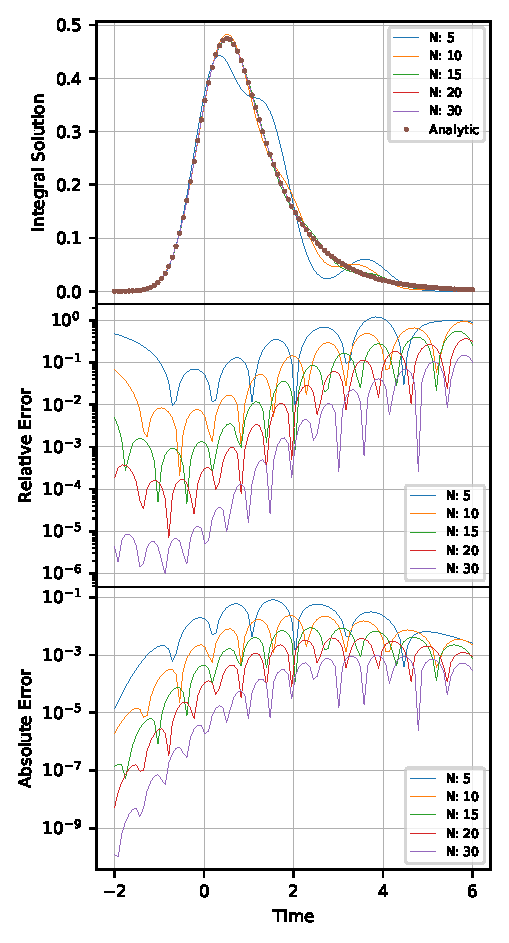
\includegraphics{CodeAndFigures/GaussLaguerreQuadrature.pdf}
    \caption{\emph{Top}: Solution to the integral of equation \ref{eq:convolution} using Gauss-Laguerre quadrature of N degrees for $\tau=1,\sigma_t=0.5$ evaluated at 100 points for $t\in[-2,6]$. \emph{Middle}: Relative error of the analytic solution and numeric solutions. \emph{Bottom}: Absolute error of the analytic solution and numeric solutions.}
    \label{fig:GaussLaguerrePlot}
\end{figure}

% %\include{name} %name without extension. insert in new page
\newpage %continues on next column
%\clearpage %continues on next page

\section{Acceptance/Rejection \\Method}

Use the Acceptance-Rejection Method to
draw random deviates from a probability distribution shaped like the first half-cycle of a sine
function (properly normalized) on the interval $[0,\pi]$.I would like you to use two different
functions for $f(x)$:
\begin{enumerate}
    \item a constant $f(x)$ for the full interval
    \item any other non-constant function of your choice.
\end{enumerate}

In each case you should compare the sine wave to a histogram your random deviates to show
that you have faithfully sampled from the distribution. Finally, for each case show that the
inefficiency factor (the number of trials you have to make divided by the number of good deviates
that you get) is equal to the area under $f(x)$ on the interval $[0,\pi]$. Note that the function that
you choose must have an efficiency factor that is smaller than that of the constant function.


\begin{table}
    \centering
    \begin{tabular}{lcc}
\toprule
{} &  Ineficiency Factor &  Total Area \\
\midrule
Constant  &                1.8776 &       1.8850 \\
Quadratic &                1.1912 &       1.1906 \\
\bottomrule
\end{tabular}

    \caption{Table that shows the total area and the inefficiency factor.}
    \label{tab:accRej}
\end{table}

\begin{figure}
  \centering
  \begin{subfigure}[b]{0.5\textwidth}
    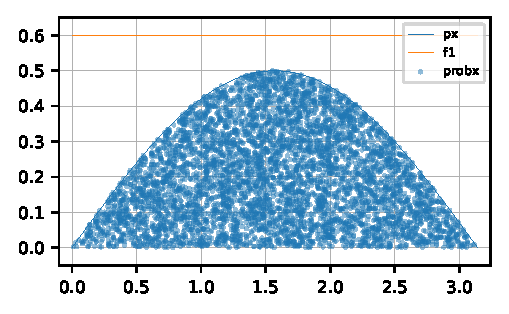
\includegraphics{CodeAndFigures/AcceptanceRejectionPlotf1.pdf}
    \caption{$f(x)=0.6$}
    \label{subfig:constant}
  \end{subfigure}
  \begin{subfigure}[b]{0.5\textwidth}
    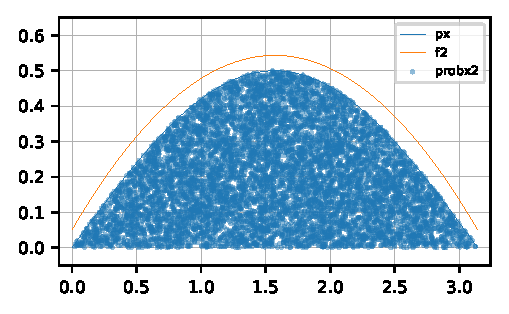
\includegraphics{CodeAndFigures/AcceptanceRejectionPlotf2.pdf}
    \caption{$f(x)=-.2x^2+.2x+.01$.}
    \label{subfig:Quadratic}
  \end{subfigure}
  \caption{Plot of random deviates from a normalized sine function using the Acceptance/Rejection Method with \ref{subfig:Quadratic} quadratic function and \ref{subfig:constant} constant function.}
  \label{fig:accRejPlot}
\end{figure}

\newpage

\section{Emcee Method}

Use the emcee python package to draw random deviates from
a probability distribution shaped like the first half-cycle of a sine function (properly normalized)
on the interval $[0,\pi]$.
\newpage

% \section{Focusing the LMT}

\subsection{}
Like all telescopes, the LMT must be focused several times a night.
To do this we make a small map of a bright point-like source and then adjust the z-position of the secondary mirror until the point spread function (the telescope’s response function) is round and maximized. 

We are given 5 maps of a point source taken on February 7, 2015. Along with them, we are given 5 other fits files which are the corresponding weights, $(1/\sigma^2)$, of the point source maps. Each map corresponds to a different z-position of the secondary mirror as shown in Table \ref{tab:LMTmaps}

We can use the Levenberg-Marquardt (LM) method \footnote{lmfit python package} to fit the point source maps to a 2D Gaussian because a point source will look as a 2D Gaussian to the telescope. The LM method is a way to minimize the $\chi^2$ function.
% using a seamless transition from the steepest descent method (STM) and the inverse Hessian method (IHM).

The point source maps can be fitted to a 2D Gaussian described by the following equation
\begin{equation}
    f(x,y)=Ae^{-a(x-x_0)^2-b(x-x_0)(y-y_0)-c(y-y_0)^2}
\end{equation}
where 
\begin{align}
    a=\frac{\cos^2\theta}{2\sigma_x^2}+\frac{\sin^2\theta}{2\sigma_y^2},\\
    b=-\frac{\sin 2\theta}{2\sigma_x^2}+\frac{\sin 2\theta}{2\sigma_y^2},\\
    c=\frac{\sin^2\theta}{2\sigma_x^2}+\frac{\cos^2\theta}{2\sigma_y^2},
\end{align}
$A$ is the amplitude, $(x_0,y_0)$ is the center of the peak, $\sigma_x,\sigma_y$ are the width of the peak and $\theta$ is a rotation angle.

Using the lmfit package we can apply the LM method to find the parameters that minimize the $\chi^2$ function for the 2D Gaussian. To do so, we first define \emph{lmfit.Model()} to use the 2D Gaussian definition specifying the independent variables $x$ and $y$, and the parameters $A,x_0,y_0,\sigma_x,\sigma_y,$ and $\theta$. After defining the model, we use \emph{lmfit.Model.fit} to fit each of the maps using the weight maps and the initial estimate of all parameters. The result are the best values of the parameters that minimizes the $\chi^2$ function. 
Figure \ref{fig:lmtRaw} shows the raw maps, the fitted map using the best values of the parameters $A,x_0,y_0,\sigma_x,\sigma_y,$ and $\theta$ and a map of the residuals, $raw-fit$. 

Once we have the best fit parameters for each map, we extract the amplitude, $A$, from each map and plot it against the z-position of the secondary mirror. This set of data will be fitted to a quadratic model described by,
\begin{equation}
    f(z)=a_0+a_1z+a_2z^2
\end{equation}
where $z$ is the z-position of the secondary mirror as given in Table \ref{tab:LMTmaps}. 

Noting that the quadratic model is linear in its parameters, we choose to do the fit using the least squares method with SVD. From this fit, we obtained the maximum and select its corresponding z-position as the best position for the secondary mirror. Figure \ref{fig:lmtquadfit} shows the amplitude and z position of the secondary mirror alongside the least squares fit using SVD and the best z-position for the secondary mirror, which for this case is \SI{-0.57}{\milli\m}.

% The data is stored in the file maps.tar.gz on the class Moodle page. You can unpack that on a linux computer with the commands: gunzip maps.tar.gz and tar -xcv maps.tar. This will give you a set of 10 fits files (remember fits from homework 1) that you will read. The files with “signal” in the name are the maps of the source. The files with "weight" in the name are images with each pixel representing the weight $(1/\sigma^2)$ of each pixel in the corresponding signal map.

% Putting all this together, use the lmfit Levenberg-Marquardt fitting package to fit each image to a 2-d gaussian. 
% Find the best fit amplitude in each case and fit the best fit amplitudes to the function
% \begin{equation}
%     f(z)=a_0+a_1z+a_2z^2
% \end{equation}
% where z is the z-position of the secondary as given in the table below.

% Use the results of this
% fit to determine the best-fit position of the LMT's secondary mirror.

\begin{table}[ht]
    \centering
    \begin{tabular}{|c|c|}
        \toprule
         Observation  & z-position (mm)  \\
         \midrule
         35114 & -3.0\\
         35115 & -2.0 \\
         35116 & -1.0 \\
         35117 & 0.0 \\
         35118 & 1.0\\
         \bottomrule
    \end{tabular}
    \caption{List of observation maps and their corresponding z-position of the secondary mirror of the LMT.}
    \label{tab:LMTmaps}
\end{table}

\begin{figure}
    \centering
    \begin{subfigure}[b]{.49\textwidth}
        \centering
        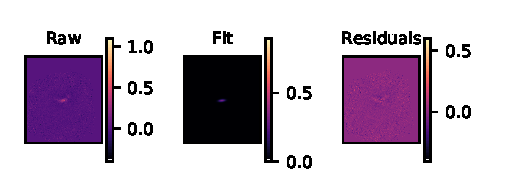
\includegraphics[height=100pt]{CodeAndFigures/DataFits4.pdf}
        \caption{Data:35114}
        \label{fig:lmtFit4}
    \end{subfigure}
    \begin{subfigure}[b]{.49\textwidth}
        \centering
        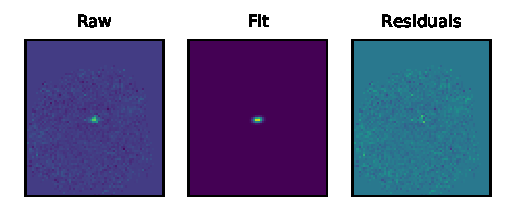
\includegraphics[height=100pt]{CodeAndFigures/DataFits5.pdf}
        \caption{Data:35115}
        \label{fig:lmtFit5}
    \end{subfigure}
    \begin{subfigure}[b]{.49\textwidth}
        \centering
        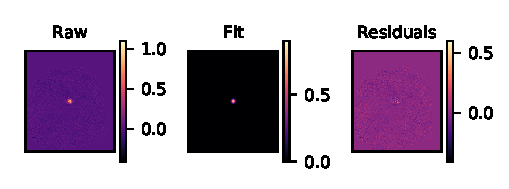
\includegraphics[height=100pt]{CodeAndFigures/DataFits6.pdf}
        \caption{Data:35116}
        \label{fig:lmtFit6}
    \end{subfigure}
    \begin{subfigure}[b]{.49\textwidth}
        \centering
        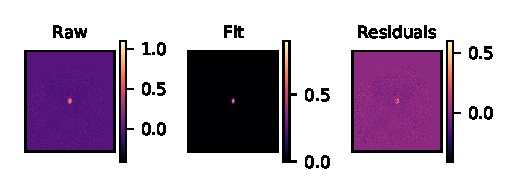
\includegraphics[height=100pt]{CodeAndFigures/DataFits7.pdf}
        \caption{Data:35117}
        \label{fig:lmtFit7}
    \end{subfigure}
    \begin{subfigure}[b]{.49\textwidth}
        \centering
        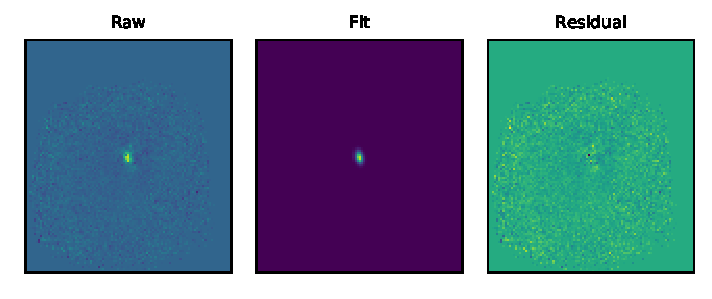
\includegraphics[height=100pt]{CodeAndFigures/DataFits8.pdf}
        \caption{Data:35118}
        \label{fig:lmtFit8}
    \end{subfigure}
    \caption{Image of the raw data, its 2D Gaussian fit and its residuals.}
    \label{fig:lmtRaw}
\end{figure}


\begin{figure}
    \centering
    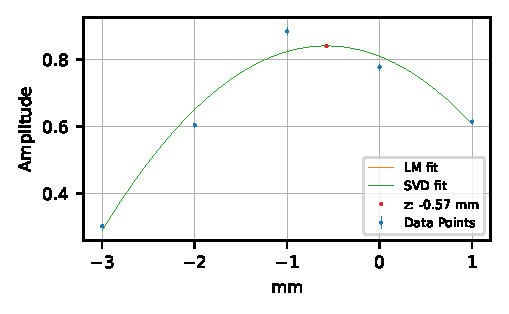
\includegraphics{CodeAndFigures/QuadFitPlot.pdf}
    \caption{Plot of the amplitude obtain by LM method from each maps vs the corresponding z-position of the secondary mirror. }
    \label{fig:lmtquadfit}
\end{figure}

\subsection{}
% Use either the procedure outlined in the class18 notes or the emcee python package to simulate the posterior probability distributions for all of the fitted parameters in one of the 2-d gaussian fits you did. Describe what you see.

We can use a posterior probability distribution of the fitted parameters to estimate the uncertainty in the fit. We start with the best fit parameters from MAP 35116 (Table \ref{tab:lmtMap2}). To do so, we do the following:
\begin{itemize}
    % \item From our data find the best fit parameters.
    \item Using the best fit parameters simulate N data sets were we randomize new parameters from normal distributions that has the best fit parameters as their mean.
    \item Find the new best fit parameters for the simulated data sets.
\end{itemize}

Figure \ref{fig:lmtpostAna} shows the posterior joint posterior probability and the marginalized posterior probability. 
We can note that our histograms for the center coordinates, rotation angle and amplitude resemble a normal distribution. 
In contrast, $\sigma_x$ and $\sigma_y$ show a double peak distribution where the maximum peak is where the best fit parameters are located. 
Nonetheless, I'm not sure what that means other than they seem to be not normal distributed.  
The rotation angle seems to be unimportant for our fit which makes sense since every 90 degrees the axis values will either flip or repeat. In addition since we are interested in maximizing the amplitude of the 2D Gaussian the rotation doesn't affect us.
Finally, the amplitude and the center coordinates are uncorrelated with each other. 

\begin{table}[ht]
    \centering
    \begin{tabular}{|c|c|}
        \toprule
         Parameter & Value  \\
         \midrule
         $x_0$       & 154.51 \\
         $y_0$       & 178.55 \\
         $\sigma_x$  & 4.35   \\
         $\sigma_y$  & 4.77   \\
         $\theta$    & 0.59   \\
         Amplitude   & 0.88   \\
         \bottomrule
    \end{tabular}
    \caption{Best fitted parameters from a 2D Gaussian for MAP 35116.}
    \label{tab:lmtMap2}
\end{table}


\begin{figure*}
    \centering
    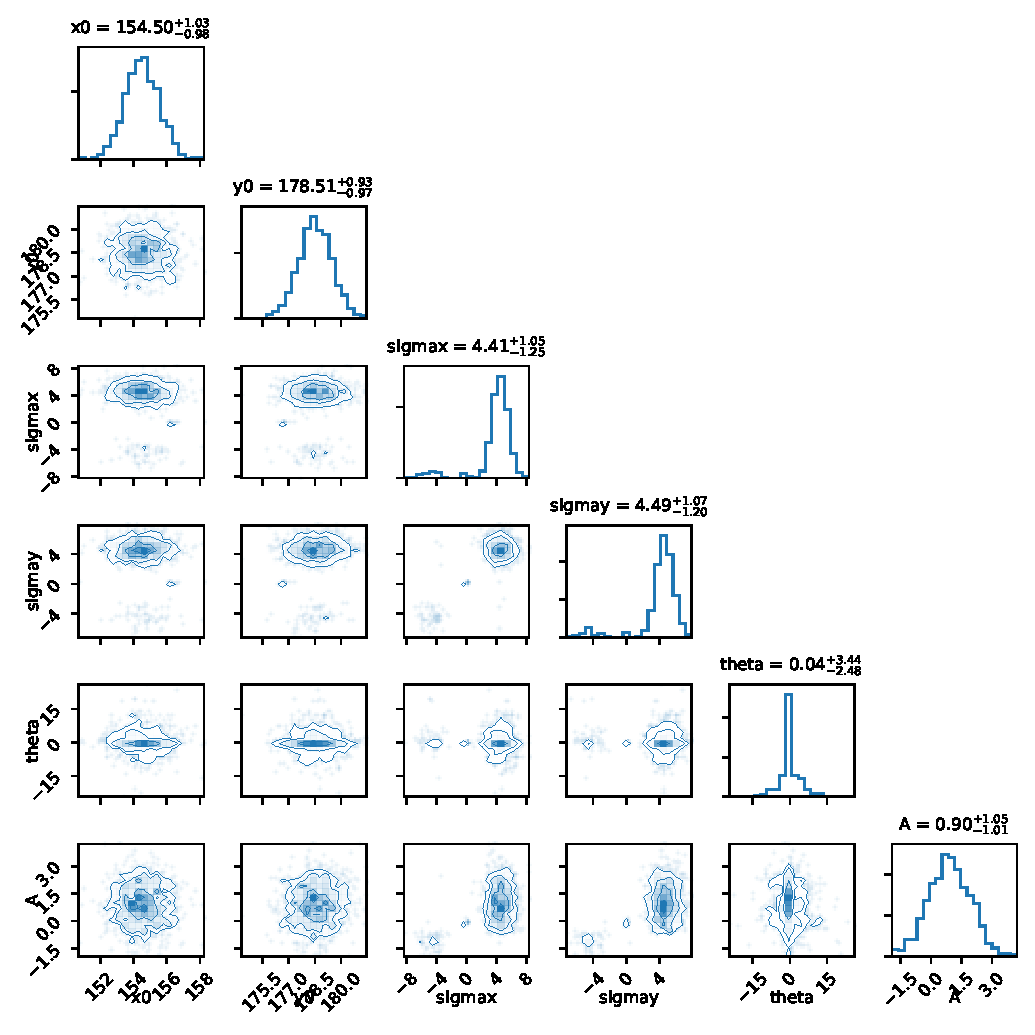
\includegraphics{CodeAndFigures/FocusingLMTPosteriorCorner.pdf}
    \caption{Posterior probability distributions for all of the fitted parameters for MAP 35116.}
    \label{fig:lmtpostAna}
\end{figure*}


% \newpage

% \section{Metropolis-Hastings \\ MCMC (linear model)}

Write a simple MetropolisHastings MCMC to fit the data from linfit data.npz to the linear function
\begin{equation}
    f(\Vec{x}|\Vec{a})=a_0 + a_1\Vec{x}
\end{equation}

Plot up the joint posterior probability distribution for the two parameters as well as marginalized posterior probabilities for each parameter. Clearly describe your process for obtaining a
good acceptance rate through tuning the average step sizes via your proposal distributions.
Overplot the joint 68.3\% and 95\% confidence intervals for the two parameters.

\begin{figure}
    \centering
    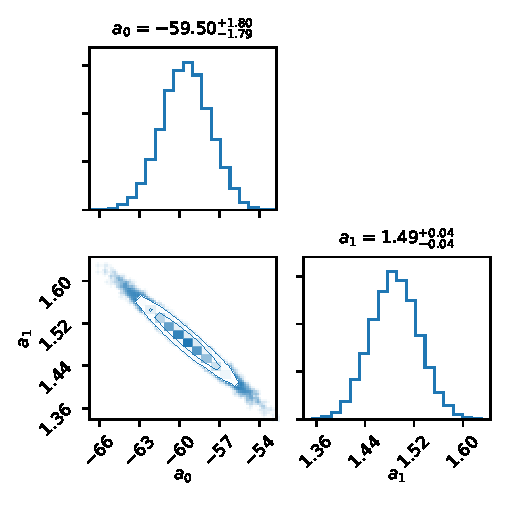
\includegraphics[0.5\textwidth]{CodeAndFigures/LinearModelMetropolisHastings.pdf}
    \caption{Caption}
    \label{fig:LinearHastings}
\end{figure}
% \newpage

% \section{Metropolis-Hastings \\MCMC (nonlinear model)}

Use the same Metropolis Hastings code to fit the data from gaussfit data.npz to the gaussian function
\begin{equation}
    f(\Vec{x}|\Vec{a})=a_0+a_1e^{-\frac{1}{2}(\frac{x-a_2}{a_3})^2}
\end{equation}

Overplot the joint 68.3\% and 95\% confidence intervals for all combinations of parameters.
%\newpage

%%%%%%%%%%%%%%%%%%%%%%%%%%%%%%%%%%%%%%%%%%%%%%%%%%%%%%%%%%%%%%%
%=====================Add Bibliography=========================
%%%%%%%%%%%%%%%%%%%%%%%%%%%%%%%%%%%%%%%%%%%%%%%%%%%%%%%%%%%%%%%

% \bibliographystyle{plain} % We choose the "plain" reference style
% %plain style sorts the reference list by alphabetical order of the first author’s last name.
% \bibliography{references} % Entries are in the "refs.bib" file

% \clearpage

% %%%%%%%%%%%%%%%%%%%%%%%%%%%%%%%%%%%%%%%%%%%%%%%%%%%%%%%%%%%%%%%
% %=====================Appendix=================================
% %%%%%%%%%%%%%%%%%%%%%%%%%%%%%%%%%%%%%%%%%%%%%%%%%%%%%%%%%%%%%%%
%  \appendix

% \section[]{Python code} 
% \lstset{caption={Astro645HW05p2.py}, style=Python}
% %\label{sec:CodeHw04p1}
% %\lstset{label={Astro732Hw04P1.py}}
% \lstinputlisting[language=Python]{CodeAndFigures/Astro645HW05p2.py}

% \newpage

% %\section[]{Python code Problem 3} 
% \lstset{caption={SetupPlots.py}, style=Python}
% \lstinputlisting[language=Python]{CodeAndFigures/SetupPlots.py}

% \newpage

% %\section[]{Python code Problem 4} 
% \lstset{caption={NumericIntegrations.py}, style=Python}
% \lstinputlisting[language=Python]{CodeAndFigures/NumericIntegrations.py}

% \newpage

% %\section[]{Python code Problem 5} 
% \lstset{caption={Astro645HW04p5.py}, style=Python}
% \lstinputlisting[language=Python]{CodeAndFigures/Astro645HW04p5.py}


\end{document}